% Created by tikzDevice version 0.6.2-92-0ad2792 on 2013-03-15 13:35:10
% !TEX encoding = UTF-8 Unicode
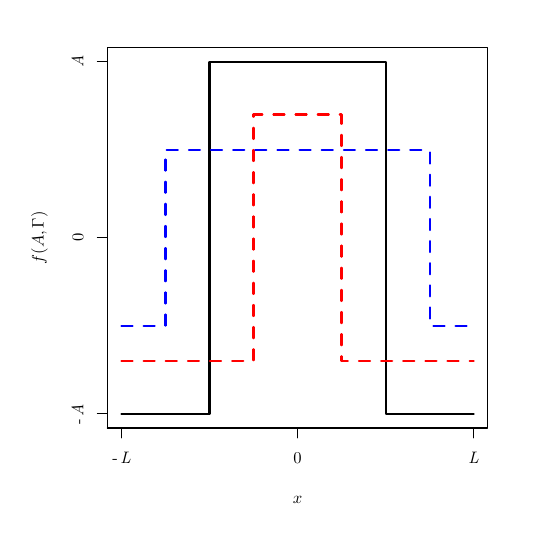
\begin{tikzpicture}[x=1pt,y=1pt, scale=0.6, every node/.style={scale=0.6}]
\definecolor[named]{fillColor}{rgb}{1.00,1.00,1.00}
\path[use as bounding box,fill=fillColor,fill opacity=0.00] (0,0) rectangle (289.08,289.08);
\begin{scope}
\path[clip] ( 48.00, 48.00) rectangle (277.08,277.08);
\definecolor[named]{drawColor}{rgb}{0.00,0.00,0.00}

\path[draw=drawColor,line width= 0.8pt,line join=round,line cap=round] ( 56.48, 56.48) --
	(109.51, 56.48) --
	(109.51,268.60) --
	(215.57,268.60) --
	(215.57, 56.48) --
	(268.60, 56.48);
\end{scope}
\begin{scope}
\path[clip] (  0.00,  0.00) rectangle (289.08,289.08);
\definecolor[named]{drawColor}{rgb}{0.00,0.00,0.00}

\path[draw=drawColor,line width= 0.4pt,line join=round,line cap=round] ( 48.00, 48.00) --
	(277.08, 48.00) --
	(277.08,277.08) --
	( 48.00,277.08) --
	( 48.00, 48.00);
\end{scope}
\begin{scope}
\path[clip] (  0.00,  0.00) rectangle (289.08,289.08);
\definecolor[named]{drawColor}{rgb}{0.00,0.00,0.00}

\node[text=drawColor,anchor=base,inner sep=0pt, outer sep=0pt, scale=  1.00] at (162.54,  2.40) {$x$};

\node[text=drawColor,rotate= 90.00,anchor=base,inner sep=0pt, outer sep=0pt, scale=  1.00] at (  9.60,162.54) {$f(A,\Gamma)$};
\end{scope}
\begin{scope}
\path[clip] (  0.00,  0.00) rectangle (289.08,289.08);
\definecolor[named]{drawColor}{rgb}{0.00,0.00,0.00}

\path[draw=drawColor,line width= 0.4pt,line join=round,line cap=round] ( 56.48, 48.00) -- (268.60, 48.00);

\path[draw=drawColor,line width= 0.4pt,line join=round,line cap=round] ( 56.48, 48.00) -- ( 56.48, 42.00);

\path[draw=drawColor,line width= 0.4pt,line join=round,line cap=round] (162.54, 48.00) -- (162.54, 42.00);

\path[draw=drawColor,line width= 0.4pt,line join=round,line cap=round] (268.60, 48.00) -- (268.60, 42.00);

\node[text=drawColor,anchor=base west,inner sep=0pt, outer sep=0pt, scale=  1.00] at ( 50.94, 26.40) {-};

\node[text=drawColor,anchor=base west,inner sep=0pt, outer sep=0pt, scale=  1.00] at ( 55.76, 26.40) {\itshape L};

\node[text=drawColor,anchor=base west,inner sep=0pt, outer sep=0pt, scale=  1.00] at (160.04, 26.40) {0};

\node[text=drawColor,anchor=base west,inner sep=0pt, outer sep=0pt, scale=  1.00] at (265.46, 26.40) {\itshape L};

\path[draw=drawColor,line width= 0.4pt,line join=round,line cap=round] ( 48.00, 56.48) -- ( 48.00,268.60);

\path[draw=drawColor,line width= 0.4pt,line join=round,line cap=round] ( 48.00, 56.48) -- ( 42.00, 56.48);

\path[draw=drawColor,line width= 0.4pt,line join=round,line cap=round] ( 48.00,162.54) -- ( 42.00,162.54);

\path[draw=drawColor,line width= 0.4pt,line join=round,line cap=round] ( 48.00,268.60) -- ( 42.00,268.60);

\node[text=drawColor,rotate= 90.00,anchor=base west,inner sep=0pt, outer sep=0pt, scale=  1.00] at ( 33.60, 50.36) {-};

\node[text=drawColor,rotate= 90.00,anchor=base west,inner sep=0pt, outer sep=0pt, scale=  1.00] at ( 33.60, 55.18) {\itshape A};

\node[text=drawColor,rotate= 90.00,anchor=base west,inner sep=0pt, outer sep=0pt, scale=  1.00] at ( 33.60,160.04) {0};

\node[text=drawColor,rotate= 90.00,anchor=base west,inner sep=0pt, outer sep=0pt, scale=  1.00] at ( 33.60,264.88) {\itshape A};
\end{scope}
\begin{scope}
\path[clip] ( 48.00, 48.00) rectangle (277.08,277.08);
\definecolor[named]{drawColor}{rgb}{1.00,0.00,0.00}

\path[draw=drawColor,line width= 0.8pt,dash pattern=on 4pt off 4pt ,line join=round,line cap=round] ( 56.48, 88.30) --
	(136.03, 88.30) --
	(136.03,236.78) --
	(189.05,236.78) --
	(189.05, 88.30) --
	(268.60, 88.30);
\definecolor[named]{drawColor}{rgb}{0.00,0.00,1.00}

\path[draw=drawColor,line width= 0.8pt,dash pattern=on 4pt off 4pt ,line join=round,line cap=round] ( 56.48,109.51) --
	( 83.00,109.51) --
	( 83.00,215.57) --
	(242.08,215.57) --
	(242.08,109.51) --
	(268.60,109.51);
\end{scope}
\end{tikzpicture}
